\chapter{Obesity associated genetic signatures and pathway signatures}
\label{cha:obesity_associated_genetic_signature_and_pathway_signatures}

In this chapter, the underlying biological mechanism of the obesity associated signatures from CR data were investigated.
In doing so, the pathway genetic signatures from the \citet{Gatza2010a} study (GT) were utilised to determine which biological pathways the obesity associated genetic signatures were most similar to.
First, the direction of GT pathway associated genetic signatures were resolved; then the pathway associated metagenes were compared with the obesity associated metagenes; and lastly linear models were constructed based on the pathway metagenes and sample \gls{bmi}/\gls{bmi} status to predict the obesity associated metagenes.

\section{Pathway associated genetic signatures from \citet{Gatza2010a} study}
\label{sec:pathway_associated_genetic_signatures_from_gatza2010a_study}

Pathway associated genetic signatures from the \citet{Gatza2010a} study were examined for their consistency with the reported results.
In the \citet{Gatza2010a} study, their data comprised of samples from different data sets from other studies, \gls{mas}-normalised and the metagene scores were ranked with probit.
However, the analyses so far have used \gls{rma}-normalisation method and ranked based on the number of samples present in the data.
To decide which normalisation or ranking methods were suitable for the analysis, the different methods were compared in GT data (see \cref{app:b}).
Results shown in \cref{app:b} clarified that there was no significant difference in the ranking methods used.
Correlation and scatter plots of the different combinations of transformation matrices (derived from either \gls{rma}- or \gls{mas}-normalised data) with \gls{rma}- or \gls{mas}-normalised data were calculated and plotted.
From these results, it seemed like the normalisation methods of the data in which the transformation matrices were applied to had the most significant effect on the resulting metagenes, rather than the transformation matrices themselves (\cref{app:b}).
This meant that all of the data sets had to be normalised with a single normalisation method, so the \gls{rma} normalisation method was used as this method was more reliable than the \gls{mas} method.
Therefore, GT data set was batch corrected first (\cref{sub:batch_correction}), then normalised with \gls{rma} method and the scores were ranked based on the number of samples in the data set.

One thing noted from these scatter plots was that there were some pathway signatures that were more variable than the others.
As an example, the \gls{tgfb} metagenes were significantly more dispersed compared to the \gls{pr} metagenes, even though both of these metagenes were generated in the same data set through similar processes (\cref{fig:gt_rma_vs_mas}).
These differences were seen in other data sets as well (\cref{app:b}).
This result provided evidence that some of the pathway genetic signatures from the \citet{Gatza2010a} study were more consistent across different data sets than the others.
\\

\begin{figure}[htpb]
	\centering
	\includegraphics[page=76,width=0.45\linewidth]{results2/allmeta_rma_vs_mas}
	\includegraphics[page=100,width=0.45\linewidth]{results2/allmeta_rma_vs_mas}
	\caption{Comparison of the metagenes generated in the \gls{mas} normalised GT data set from the application of the transformation matrices derived from either the \gls{rma} or \gls{mas} normalised data}
	\label{fig:gt_rma_vs_mas}
\end{figure}

\noindent
Before GT pathway metagenes were compared with the obesity associated metagenes, the direction of GT pathway metagenes had to be checked to make sure the metagenes were in the correct direction (\cref{sub:metagene_direction}).
% Each pathway metagenes was generated from GT data set and the direction of the metagene was checked with the expression of the representative pathway gene (\cref{tab:metagene_direction}), and the groupings of the pathways were considered as well.
The correlation of all the pathway metagenes with one another were plotted as a heatmap in \cref{fig:gatza_meta_dir}.
The most prominent group had five pathways (E2F1, \gls{pi3k}, Myc, \gls{bcat} and Ras) that clustered at the top right hand corner of the heatmap.
% TODO: add additional info about why these pathways clustered together?
Other groups included \gls{ifna}/\gls{ifny}/\gls{tnfa} pathways, \gls{er}/\gls{pr}/p53 pathway and p63/\gls{her2} pathways.
In addition to these highly correlated groups, \gls{stat3}/\gls{tgfb}/Src/\gls{egfr}/Akt pathways showed little correlation with one another.
Comparing these groups with the results presented by \citet{Gatza2010a} (see \cref{app:b}), the identified groups approximately resembled the groups identified in their study, which confirmed that the directions of GT pathway metagenes were similar to those used by Gatza \textit{et al.}.

\begin{figure}[htpb]
	\centering
	\includegraphics[page=15,width=0.7\linewidth]{results2/gatza_meta_trans}
	\caption{Heatmap of all the pathway metagenes from the \citet{Gatza2010a} study in GT data set}
	\label{fig:gatza_meta_dir}
\end{figure}

To see whether the directionality of GT pathway metagenes were being transferred across to other data sets properly, pathway metagenes were generated in other data sets with the transformation matrices and the groupings of the metagenes were examined.
CR, FM and \gls{nzbc} data were \gls{rma}-normalised and transformation matrices of the pathway genetic signatures (derived from GT data set) were applied to the data sets.
The metagenes were plotted in a heatmap (shown in \cref{app:b}), which showed similar groupings  as seen in \cref{fig:gatza_meta_dir}.
This result confirmed that the pathway metagenes were acting similarly in all the data sets in which the transformation matrices have been applied to.

% In order to investigate what the underlying biological mechanism of the obesity associated genetic signatures was, GT pathway associated genetic signatures were used to create linear models to predict the obesity associated metagene scores.
% Before linear models were created, GT pathway metagenes were checked for their directionality to ensure that the pathway metagenes were acting as reported by \citet{Gatza2010a} (see \cref{sub:metagene_direction}).

\section{Pathway associated metagenes and obesity associated metagenes}
\label{sec:pathway_associated_metagenes_and_obesity_associated_metagenes}

Results from previous section confirmed that the pathway metagenes from the \citet{Gatza2010a} study were in the correct directions, and that the pathway metagenes were behaving as expected in different data sets.
Now that the directions of the pathway metagenes were established, these metagenes were ready for comparison with the obesity associated metagenes.
However, all of the pathway metagenes were derived from GT data, whereas the majority of the obesity associated metagenes were derived from CR data, which presents a problem of deciding on which data set the transformation matrices should be generated in.

In theory, the metagenes generated from the application of \gls{svd} and the metagenes generated from transformation matrix would be exactly the same if the transformation matrix was derived from the same data set.
For example, an obesity associated metagene generated from CR data with \gls{svd} would have the same values as the metagenes generated in CR data with the transformation matrix (where the transformation matrix was derived from CR data).
Furthermore, if the \gls{svd}-derived metagenes and transformation matrix-derived metagenes were the same (or at least similar) in a different data set, this suggests that there was no difference in the data sets, at least in terms of the expression of the genetic signatures being investigated.
In other words, the transformation matrix can be made in either the original data set or in a different data set if there was no difference in the \gls{svd}-derived or transformation matrix-derived metagenes.

To decide which data set the transformation matrices for obesity and pathway associated genetic signatures should be generated in, the \gls{svd}- and transformation matrix(TM)-generated metagene scores were compared in all of the data sets.
As in \cref{sec:pathway_associated_genetic_signatures_from_gatza2010a_study}, all data sets were normalised with the \gls{rma} method and metagenes were ranked based on the number of samples in each data set.
Transformation matrices for the obesity associated genetic signatures were made in CR data set and pathway associated genetic signatures were made in GT data set.
Metagenes for all of the obesity and pathway associated genetic signatures were generated in all of the data sets with \gls{svd} and transformation matrices.
The Spearman correlation of the \gls{svd}-generated and TM-generated metagene scores were calculated for each genetic signatures (\cref{tab:svd_vs_tm_path,tab:svd_vs_tm_obs}).

\begin{table}[htpb]
	\centering
	\begin{threeparttable}
	\caption{Summary of the Spearman correlations of the pathway metagenes generated from \gls{svd} and the application of the transformation matrices\tnote{1} in GT, CR, \gls{nzbc} and FM data sets}
	\label{tab:svd_vs_tm_path}
		\begin{tabular}{lcccc}
			& GT & CR & \gls{nzbc} & FM\\
			\hline
			\hline
			\rule{0pt}{2.25ex}Akt & 1.000 & 0.5190 & 0.5900 & 0.5563 \\
			\gls{bcat}            & 1.000 & 0.9897 & 0.9977 & 0.9905 \\
			E2F1                  & 1.000 & 0.9646 & 0.8438 & 0.9193 \\
			\gls{egfr}            & 1.000 & 0.0430 & 0.3358 & 0.4040 \\
			\gls{er}              & 1.000 & 0.9978 & 0.9942 & 0.9966 \\
			\gls{her2}            & 1.000 & 0.9553 & 0.5817 & 0.9794 \\
			\gls{ifna}            & 1.000 & 0.9830 & 0.9991 & 0.9951 \\
			\gls{ifny}            & 1.000 & 0.9086 & 0.9950 & 0.9718 \\
			Myc                   & 1.000 & 0.9878 & 0.9852 & 0.9689 \\
			p53                   & 1.000 & 0.3808 & 0.9981 & 0.7923 \\
			p63                   & 1.000 & 0.8319 & 0.2951 & 0.8368 \\
			\gls{pi3k}            & 1.000 & 0.9543 & 0.5989 & 0.9365 \\
			\gls{pr}              & 1.000 & 0.9511 & 0.9887 & 0.9845 \\
			Ras                   & 1.000 & 0.9078 & 0.9125 & 0.7229 \\
			Src                   & 1.000 & 0.9575 & 0.7173 & 0.9548 \\
			\gls{stat3}           & 1.000 & 0.1902 & 0.9159 & 0.6167 \\
			\gls{tgfb}            & 1.000 & 0.9918 & 0.2543 & 0.9890 \\
			\gls{tnfa}            & 1.000 & 0.6046 & 0.9365 & 0.4315 \\
			\hline
			\hline
		\end{tabular}
		\begin{tablenotes}
			\begin{footnotesize}
				\item [1] Transformation matrices were derived from the GT data set.
			\end{footnotesize}
		\end{tablenotes}
	\end{threeparttable}
\end{table}

\begin{table}[htpb]
	\centering
	\begin{threeparttable}
		\caption{Summary of the Spearman correlations of the obesity metagenes generated from \gls{svd} and the application of the transformation matrices\tnote{1} in GT, CR, \gls{nzbc} and FM data sets}
		\label{tab:svd_vs_tm_obs}
		\begin{tabular}{lcccc}
			& CR & GT & FM & \gls{nzbc}\\
			\hline
			\hline
			\rule{0pt}{2.25ex} Cr & 1.000     & 0.9985 & 0.9872 & 0.9161 \\
			Res                   & 1.000     & 0.9987 & 0.9898 & 0.9652 \\
			CrOl                  & 1.000     & 0.9982 & 0.9926 & 0.9715 \\
			ResOl                 & 1.000     & 0.9981 & 0.9927 & 0.9571 \\
			Ca                    & 1.000     & 0.9985 & 0.9893 & 0.9468 \\
			CaRes                 & 1.000     & 0.9988 & 0.9939 & 0.9865 \\
			CaOl                  & 1.000     & 0.9983 & 0.9937 & 0.9677 \\
			CaResOl               & 1.000     & 0.9984 & 0.9952 & 0.9642 \\
			Original              & 1.000     & 0.9928 & 0.9862 & 0.9344 \\
			\hline
			\hline
		\end{tabular}
			\begin{tablenotes}
				\begin{footnotesize}
				\item [1] Transformation matrices were derived from the CR data set.
				\end{footnotesize}
			\end{tablenotes}
	\end{threeparttable}
\end{table}

In \cref{tab:svd_vs_tm_path,tab:svd_vs_tm_obs}, the obesity and pathway associated genetic signatures had a correlatin of 1 in CRs and GT data sets respectively, as the transformation matrices were generated in those data sets.
The correlations of the obesity and pathway metagenes were variable across different data sets, which was as expected since all the data sets were different from one another.
However, what was unexpected was the fact that there were some genetic signatures that were highly correlated in all of the data sets, whereas the metagene correlation of other signatures were highly variable across different data sets.
For example, the \gls{bcat} pathway metagene was highly correlated in all of the data sets (\textgreater{} 0.98), whereas the \gls{stat3} pathway metagene was variable across different data sets, ranging from 0.1902 to 0.9159 (\cref{tab:svd_vs_tm_path,fig:allmetacor_bar}).
The fact that some pathway associated metagenes were consistent across different data sets suggested that some of these genetic signatures were reliable and did not depend on the data set the transformation matrices were derived from.
On the other hand, the genetic signatures that were not consistent across the data sets were likely to be dependent on the data set in which they were derived from, and therefore the transformation matrices for these signatures must be derived from GT data set.

In contrast to the pathway associated genetic signatures, all of the obesity associated genetic signatures showed high correlation of the \gls{svd}- and transformation matrix-generated metagenes across the different data sets.
This suggested that obesity associated genetic signatures were consistent across all data sets and the transformation matrices for these signatures could be made in any of the data sets.
Taken together, transformation matrices for all the genetic  signatures were decided to be made in the GT data set, since there were some pathway associated signatures that were specific to GT data, but none of the obesity associated genetic signatures were specific to a data set.
\\

\begin{figure}[htpb]
	\centering
	\includegraphics[page=2,width=0.45\linewidth]{results2/allmetacor_bar}
	\includegraphics[page=16,width=0.45\linewidth]{results2/allmetacor_bar}
	\caption{Visual comparison of the Spearman correlations of \gls{svd}-derived and transformation matrix-derived \gls{bcat} and \gls{stat3} metagenes across different data sets}
	\label{fig:allmetacor_bar}
\end{figure}

\noindent
To visually determine which pathway associated genetic signatures were most similar to the obesity associated genetic signatures, heatmaps were created with the metagenes for all of the genetic signatures.
The directions of the pathway associated metagenes have already been determined in \cref{sec:pathway_associated_genetic_signatures_from_gatza2010a_study}, and the directions of the obesity associated metagenes were checked in GT data set as described in \cref{sub:metagene_direction}.
All of the metagenes were created in \gls{rma}-normalised GT data set with \gls{svd}, and the metagene scores were plotted in a heatmap and clustered into groups (\cref{fig:gatza_allmeta}).

\begin{figure}[htpb]
	\centering
	\includegraphics[page=15,width=0.8\linewidth]{results2/all_meta_trans}
	\caption{Heatmap of all the pathway and obesity metagenes in GT data set}
	\label{fig:gatza_allmeta}
\end{figure}

From \cref{fig:gatza_allmeta}, all of the obesity associated metagenes from CR data set clustered together into a group, but none of the pathway associated metagenes associated strongly with the obesity metagenes.
Though \gls{her2} and p63 pathway metagenes were grouped next to the cluster of obesity metagenes, the similarity was at most about 0.6.
FM obesity associated metagene did not cluster together with the obesity metagenes from CR data set, nor with any of the other pathway metagenes.
The fact that FM metagene did not cluster with any of the CR metagenes showed that the nature of FM metagene was different from those metagenes found in CR data set.
Furthermore, their metagene did not cluster with the Akt pathway in the heatmap, even though \citet{Fuentes-Mattei2014} provided clear evidence that their metagene specifically activated the Akt/\gls{mtor} signalling pathway in a mouse model.
This may have been due to the lack of consistency of the Akt pathway signature in different data sets (\cref{tab:svd_vs_tm_path}).
Another likely reason could be that FM genetic signature was not comprised only of the genes from the Akt pathway, but genes from other pathways as well, and so the metagene did not cluster together with the Akt pathway signature in the heatmap.

The results in this section suggested that none of the obesity associated genetic signatures were similar or related to any of the pathway associated genetic signatures from the \citet{Gatza2010a} study.

(add heatmaps of other data (Creighton/FM/Cris) as well? or maybe in appendix)

\section{Prediction of obesity associated metagenes with pathway associate metagenes}
\label{sec:prediction_of_obesity_associated_metagene_with_pathway_associate_metagene}

% and lastly linear models were constructed based on the pathway metagenes and sample \gls{bmi}/\gls{bmi} status to predict the obesity associated metagenes.

To confirm that the obesity associated metagenes were not related to any of the biological pathway signatures from the \citet{Gatza2010a} study, linear models were created to predict the obesity metagene scores with the pathway metagene scores.
If any of the pathway metagenes were significant in the linear model, this provided evidence that the significant pathways in the linear model were related to the obesity metagene.
Since most of the obesity metagenes were found in CR data set and only CR and \gls{nzbc} data sets had \gls{bmi}/\gls{bmi} status information for the samples, \gls{nzbc} data set was used as the training data set to create linear models for obesity metagene score prediction.

Metagene scores used for the construction of linear models were generated from the application of the transformation matrices derived from GT data (from \cref{sec:pathway_associated_metagenes_and_obesity_associated_metagenes}) to \gls{rma}-normalised \gls{nzbc} data.
For each of the obesity metagenes identified, seven linear models were created: \gls{bmi}-only, \gls{bmi} status-only, \gls{bmi} and \gls{bmi} status, pathway metagenes-only, and all of the combinations of pathway metagenes with \gls{bmi} and/or \gls{bmi} status.
The only variables that showed significance in any of the models that predicted the obesity metagenes taken from the CR data set were \gls{pr} metagene and whether samples were obese or not (\cref{tab:lm_sig_var}).
In the model that predicted the FM metagene scores, the obesity status of the samples and Myc metagene score were significant, but the \gls{pr} metagene score was not (\cref{app:b}).

\begin{table}[htpb]
	\centering
	\caption{Description of the linear models used to predict the Cr obesity metagene in \gls{nzbc} data set}
	\label{tab:lm_sig_var}
	\begin{threeparttable}
		\begin{tabular}{llrr}
			Linear Model & Variables & Estimate & P-value\\
			\hline
			\hline
			\rule{0pt}{2.25ex}\gls{bmi} only                           & \gls{bmi}  & -0.0016 & 0.717\\
			\hline
			\rule{0pt}{2.25ex}\gls{bmi} status only                    & Overweight & -0.0126 & 0.871\\
                                                                       & Obese      & -0.0981 & 0.166\\
			\hline
			\rule{0pt}{2.25ex}\gls{bmi} and \gls{bmi} status           & \gls{bmi}  & 0.0109  & 0.123\\
                                                                       & Overweight & -0.0687 & 0.420\\
                                                                       & Obese      & -0.2481 & \textbf{0.040}\tnote{1}\\
			\hline
			\rule{0pt}{2.25ex}Pathways only                            & \gls{bcat} & 0.0916  & 0.677\\
                                                                       & \gls{er}   & 0.0523  & 0.834\\
                                                                       & \gls{ifna} & -0.4993 & 0.307\\
                                                                       & \gls{ifny} & 0.4224  & 0.398\\
                                                                       & Myc        & -0.0038 & 0.987\\
                                                                       & \gls{pr}   & 0.5836  & \textbf{0.016}\\
			\hline
			\rule{0pt}{2.25ex}\gls{bmi} and Pathways                   & \gls{bmi}  & -0.0024 & 0.527\\
                                                                       & \gls{bcat} & 0.1121  & 0.614\\
                                                                       & \gls{er}   & 0.0540  & 0.829\\
                                                                       & \gls{ifna} & -0.5383 & 0.276\\
                                                                       & \gls{ifny} & 0.4661  & 0.358\\
                                                                       & Myc        & 0.0168  & 0.941\\
                                                                       & \gls{pr}   & 0.5927  & \textbf{0.015}\\
			\hline
			\rule{0pt}{2.25ex}\gls{bmi} status and Pathways            & Overweight & -0.0120 & 0.864\\
                                                                       & Obese      & -0.1035 & 0.113\\
                                                                       & \gls{bcat} & 0.1495  & 0.501\\
                                                                       & \gls{er}   & 0.0326  & 0.896\\
                                                                       & \gls{ifna} & -0.6707 & 0.177\\
                                                                       & \gls{ifny} & 0.5888  & 0.245\\
                                                                       & Myc        & 0.0439  & 0.846\\
                                                                       & \gls{pr}   & 0.5799  & \textbf{0.016}\\
			\hline
			\rule{0pt}{2.25ex}\gls{bmi}, \gls{bmi} status and pathways & \gls{bmi}  & 0.0091  & 0.161\\
                                                                       & Overweight & -0.0576 & 0.455\\
                                                                       & Obese      & -0.2292 & \textbf{0.040}\\
                                                                       & \gls{bcat} & 0.1460  & 0.509\\
                                                                       & \gls{er}   & 0.0091  & 0.971\\
                                                                       & \gls{ifna} & -0.6937 & 0.161\\
                                                                       & \gls{ifny} & 0.5890  & 0.243\\
                                                                       & Myc        & 0.0263  & 0.907\\
                                                                       & \gls{pr}   & 0.5449  & \textbf{0.024}\\
			\hline
			\hline
		\end{tabular}
		\begin{tablenotes}
			\begin{footnotesize}
				\item [1] All values in bold are statistically significant (p \textless{} 0.05).
			\end{footnotesize}
		\end{tablenotes}
	\end{threeparttable}
\end{table}

All of the models constructed from sample \gls{bmi}, \gls{bmi} status and/or GT pathway metagene scores confirmed that none of the pathways were significant, except for the \gls{pr} and Myc pathway metagene scores in the models for CR metagenes and FM metagene, respectively.
It was not surprising that the \gls{pr} pathway metagene showed significance in the models generated in \gls{nzbc} data set, as \gls{pr} status was very strongly correlated with \gls{nzbc} data set.
The significance of the Myc metagene in the model for FM metagene was difficult to interpret, as there was no reported association of FM metagene with Myc pathway by \citet{Fuentes-Mattei2014}.
However, ``sustained cell proliferation'' was one of the cancer hallmarks that \citet{Fuentes-Mattei2014} had shown to be related to their obesity genetic signature, so the Myc pathway metagene may have picked up the proliferation signal in the FM metagene.

Since the \gls{pr} pathway metagene showed significant association in many of the linear models, linear models were made with each of the combinations of \gls{bmi}, \gls{bmi} status and \gls{pr} pathway metagene for all of the obesity associated metagenes (\cref{tab:lm_pr_only} and \cref{app:b}).
As expected, all of the linear models showed significant contribution of the \gls{pr} metagene scores to the model for all obesity metagenes (except FM metagene; \cref{app:b}).

\begin{table}[htpb]
	\centering
	\caption{Description of the linear models used to predict the Cr obesity metagene in \gls{nzbc} data set, using only the sample \gls{bmi}, \gls{bmi} status and \gls{pr} pathway metagene scores}
	\label{tab:lm_pr_only}
	\begin{threeparttable}
			\begin{tabular}{llr{\bfseries}S}
				Linear Model & Variables & Estimate & {P-value}\\
				\hline
				\hline
				\rule{0pt}{2.25ex}\gls{pr} only                            & \gls{pr}   & 0.477  & {\bfseries \num{6.06d-7}}\tnote{1}\\
				\hline
				\rule{0pt}{2.25ex}\gls{bmi} and \gls{pr}                   & \gls{bmi}  & -0.002 & 0.586\\
                                                                           & \gls{pr}   & 0.478  & {\bfseries \num{6.35d-7}}\\
				\hline
				\rule{0pt}{2.25ex}\gls{bmi} status and \gls{pr}            & Obese      & -0.085 & 0.176\\
                                                                           & Overweight & -0.011 & 0.875\\
                                                                           & \gls{pr}   & 0.471  & {\bfseries \num{8.25d-7}}\\
				\hline
				\rule{0pt}{2.25ex}\gls{bmi}, \gls{bmi} status and \gls{pr} & \gls{bmi}  & 0.007  & 0.237\\
                                                                           & Obese      & -0.188 & 0.081\\
                                                                           & Overweight & -0.049 & 0.516\\
                                                                           & \gls{pr}   & 0.459  & {\bfseries \num{1.54d-6}}\\
				\hline
				\hline
			\end{tabular}
			\begin{tablenotes}
				\begin{footnotesize}
					\item [1] All values in bold are statistically significant (p \textless{} 0.05).
				\end{footnotesize}
			\end{tablenotes}
	\end{threeparttable}
\end{table}

To determine whether any of the linear models were able to predict the corresponding obesity metagene scores, the predicted metagene scores were generated from the models and then compared with the original scores.
The predictions were first made in \gls{nzbc} data, where the metagene scores generated from the application of transformation matrices (from GT data set) were used to make the predictions.
The predicted metagenes were then compared with the true metagenes that were originally generated from the transformation matrices (\cref{fig:predict_cris_cris}).

The predicted metagenes from the \gls{bmi} only, \gls{bmi} status only and \gls{bmi} and \gls{bmi} status linear models were not significantly related to the true metagene in many of the obesity metagenes; though \gls{bmi} and \gls{bmi} status model showed significance in some metagenes (\cref{app:b}).
On the other hand, all of the predicted metagenes generated from the models that contained any of the pathway metagenes showed significant association with the true metagene scores in all of the obesity metagenes (\cref{fig:predict_cris_cris,app:b}).
However, the $R^2$ values for all of the predicted metagenes against the true metagenes were very low ($R^2$ \textless{} 0.4).
Furthermore, all of the plots in \cref{fig:predict_cris_cris,app:b} showed clearly that the data points in the scatter plots were highly variable, suggesting that even though the association between the predicted and the true metagene scores were statistically significant, the variables in the linear models may not be strongly associated to the obesity metagene.

\begin{figure}[htpb]
	\centering
	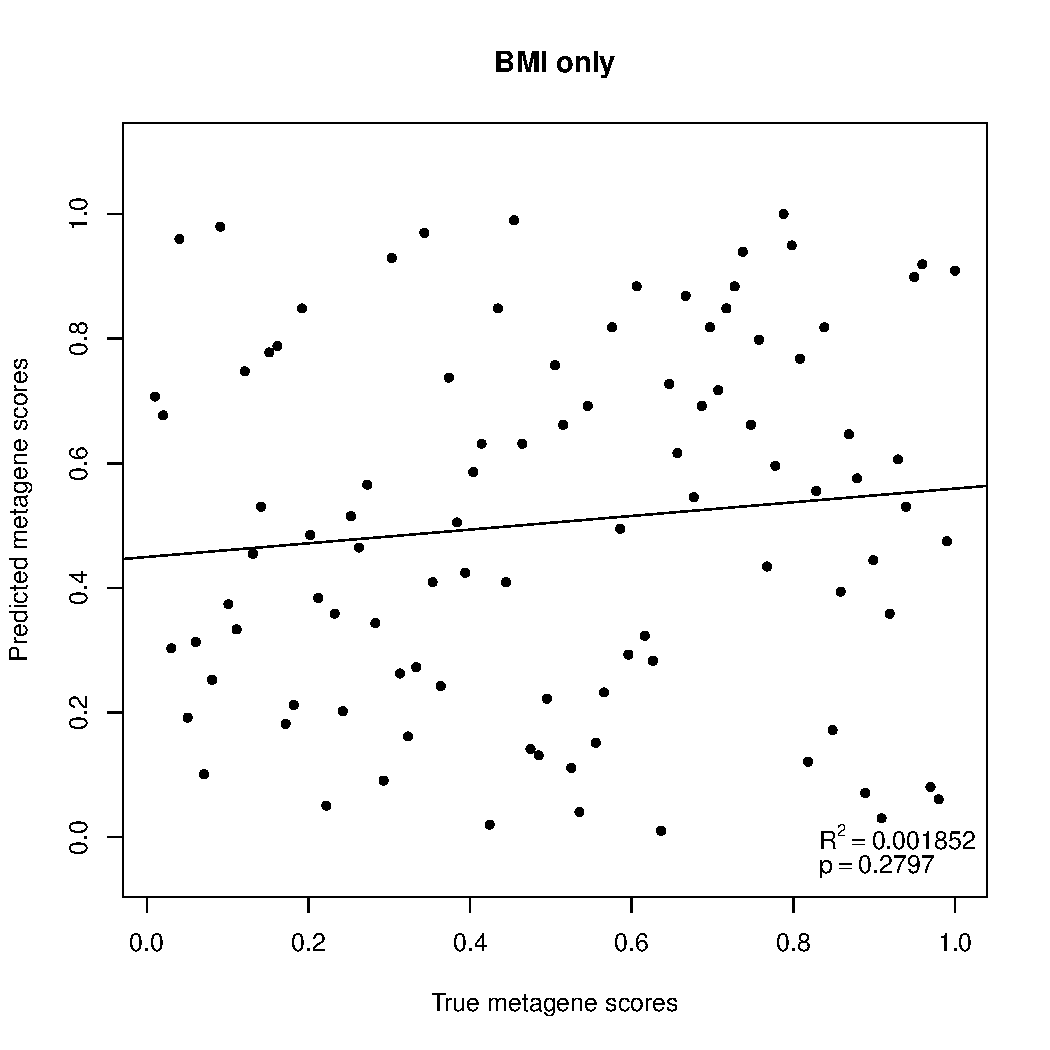
\includegraphics[page=1,width=0.32\linewidth]{results2/prediction_cris_with_cris(cris_model)}
	\includegraphics[page=2,width=0.32\linewidth]{results2/prediction_cris_with_cris(cris_model)}
	\includegraphics[page=3,width=0.32\linewidth]{results2/prediction_cris_with_cris(cris_model)}
	\includegraphics[page=4,width=0.32\linewidth]{results2/prediction_cris_with_cris(cris_model)}
	\includegraphics[page=5,width=0.32\linewidth]{results2/prediction_cris_with_cris(cris_model)}
	\includegraphics[page=6,width=0.32\linewidth]{results2/prediction_cris_with_cris(cris_model)}
	\includegraphics[page=7,width=0.32\linewidth]{results2/prediction_cris_with_cris(cris_model)}
	\includegraphics[page=74,width=0.32\linewidth]{results2/prediction_cris_with_cris(cris_model)}
	\includegraphics[page=71,width=0.32\linewidth]{results2/prediction_cris_with_cris(cris_model)}
	\includegraphics[page=72,width=0.32\linewidth]{results2/prediction_cris_with_cris(cris_model)}
	\includegraphics[page=73,width=0.32\linewidth]{results2/prediction_cris_with_cris(cris_model)}
	\caption{Comparison of the predicted Cr metagenes with the true Cr metagene in the \gls{nzbc} data}
	\label{fig:predict_cris_cris}
\end{figure}

To confirm the results shown in \gls{nzbc} data set (training set), the linear models were applied to CR data (test set).
As shown in \cref{fig:predict_cr_cris}, all of the predicted metagenes generated from the linear models were statistically significantly associated with the true metagenes, although there were some exceptions in the models for other obesity metagenes (see \cref{app:b}).
Similar to the results from \gls{nzbc} data set, all of the $R^2$ values were low ($R^2$ \textless{} 0.43) and the data points were widely spread out in the plots.
Again, these results suggested that the predicted metagene scores from the linear models may be statistically significant, but may not be relevant to the obesity metagenes which the models predict, as the predicted values were only weakly associated with the true values.
\\

\begin{figure}[htpb]
	\centering
	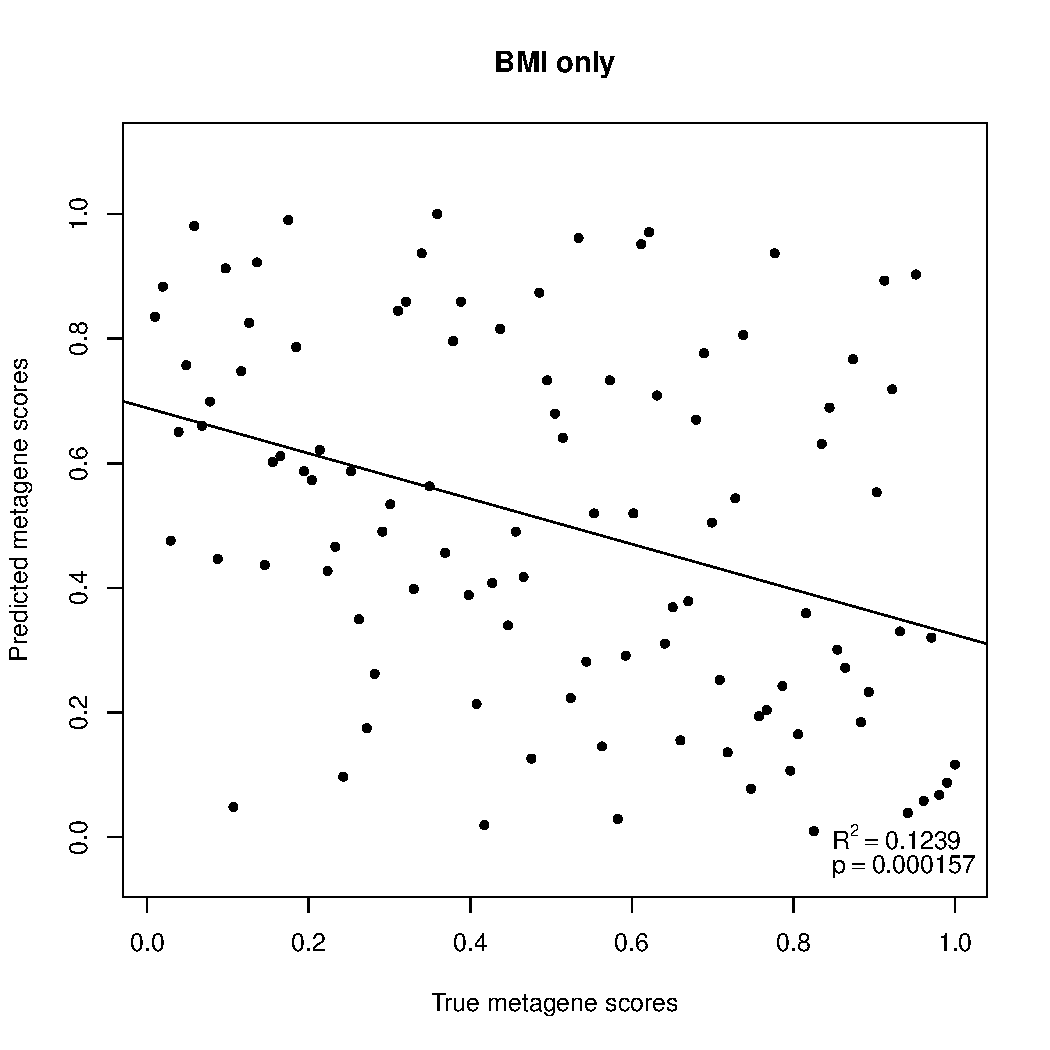
\includegraphics[page=1,width=0.32\linewidth]{results2/prediction_cr_with_cris}
	\includegraphics[page=2,width=0.32\linewidth]{results2/prediction_cr_with_cris}
	\includegraphics[page=3,width=0.32\linewidth]{results2/prediction_cr_with_cris}
	\includegraphics[page=4,width=0.32\linewidth]{results2/prediction_cr_with_cris}
	\includegraphics[page=5,width=0.32\linewidth]{results2/prediction_cr_with_cris}
	\includegraphics[page=6,width=0.32\linewidth]{results2/prediction_cr_with_cris}
	\includegraphics[page=7,width=0.32\linewidth]{results2/prediction_cr_with_cris}
	\includegraphics[page=74,width=0.32\linewidth]{results2/prediction_cr_with_cris}
	\includegraphics[page=71,width=0.32\linewidth]{results2/prediction_cr_with_cris}
	\includegraphics[page=72,width=0.32\linewidth]{results2/prediction_cr_with_cris}
	\includegraphics[page=73,width=0.32\linewidth]{results2/prediction_cr_with_cris}
	\caption{Comparison of the predicted Cr metagenes with the true Cr metagene in the CR data}
	\label{fig:predict_cr_cris}
\end{figure}

\noindent
Lastly, since only the ``consistent'' pathway metagenes were picked from all of the available pathway metagene scores, linear models were constructed with all of the pathway metagenes in a step wise fashion.
Step wise construction of a linear model is where the variables for a model are selected computationally depending on the contribution of the variable to the resuting linear model, and thus contains only the variables that ``matter'' to the linear model.
Sample \gls{bmi}, \gls{bmi} status and all of the pathway metagene scores were used to generate the step wise linear model for each of the obesity metagenes.
The linear models that resulted from the step wise selection of the variables were summarised in \cref{tab:stepwise_model}.

\begin{longtable}{llr{\bfseries}S}
	\centering
	\caption{Description of the step wise linear models used to predict all of the obesity metagenes in \gls{nzbc} data set}
	\label{tab:stepwise_model}\\
		Obesity metagene & Variables used in the model & Estimate & {P-value}\\
		\hline
	\endfirsthead
	\multicolumn{4}{c}{\tablename\ \thetable{}\ (continued)}\\
		\hline
		\hline
	\endhead
		\hline
		\hline
		Cr         & Akt         & -0.3415   & \bfseries \num{4.43d-8}\\
				   & \gls{egfr}  & 0.33852   & \bfseries \num{1.94d-05}\\
				   & \gls{er}    & -0.20237  & \bfseries 0.00419\\
				   & \gls{ifny}  & 0.12233   & 0.08700\\
				   & \gls{pr}    & -0.33920  & \bfseries \num{2.09d-5}\\
				   & Ras         & -0.22611  & \bfseries 0.00193\\
				   & Src         & -0.11452  & 0.08177\\
				   & \gls{tgfb}  & 0.55638   & \bfseries \textless{} \num{2d-16}\\
				   & \gls{tnfa}  & -0.25501  & \bfseries 0.00616\\
		\hline
		CrOl       & Overweight  & 0.040918  & 0.074865\\
				   & Obese       & -0.006381 & 0.756121\\
				   & Akt         & -0.356713 & \bfseries \num{1.89d-07}\\
				   & E2F1        & 0.160229  & \bfseries 0.005411\\
				   & \gls{egfr}  & 0.148618  & 0.062683\\
				   & p53         & 0.336552  & \bfseries \num{4.35d-05}\\
				   & \gls{pr}    & -0.225423 & \bfseries 0.000639\\
				   & Src         & -0.428758 & \bfseries \num{5.85d-10}\\
				   & \gls{stat3} & -0.124118 & \bfseries 0.009658\\
		\hline
		Res        & Akt         & 0.24613   & \bfseries 0.000289\\
				   & \gls{egfr}  & -0.46827  & \bfseries \num{2.16d-05}\\
				   & \gls{er}    & 0.18400   & 0.061446\\
				   & \gls{her2}  & 0.13835   & 0.118228\\
				   & \gls{ifny}  & -0.21019  & \bfseries 0.044084\\
				   & \gls{pr}    & 0.41195   & \bfseries 0.000300\\
				   & Ras         & 0.26506   & \bfseries 0.010465\\
				   & \gls{tgfb}  & -0.58075  & \bfseries \num{7.64d-11}\\
				   & \gls{tnfa}  & 0.42200   & \bfseries 0.001834\\
		\hline
		ResOl      & Akt         & -0.33596  & \bfseries 0.000294\\
				   & \gls{bcat}  & -0.19866  & 0.138953\\
				   & E2F1        & 0.36059   & \bfseries 0.009325\\
				   & \gls{egfr}  & 0.23421   & 0.056865\\
				   & \gls{her2}  & -0.13652  & 0.121689\\
				   & p53         & 0.38746   & \bfseries 0.000519\\
				   & \gls{pi3k}  & -0.21881  & 0.148676\\
				   & \gls{pr}    & -0.32228  & \bfseries 0.001656\\
				   & Ras         & -0.28984  & \bfseries 0.033975\\
				   & Src         & -0.40779  & \bfseries \num{5.26d-06}\\
				   & \gls{stat3} & -0.11452  & 0.125609\\
				   & \gls{tnfa}  & -0.11442  & 0.117023\\
		\hline
		Ca         & Akt         & -0.26243  & \bfseries \num{7.04d-06}\\
				   & \gls{egfr}  & 0.36305   & \bfseries 0.000139\\
				   & \gls{er}    & -0.18614  & \bfseries 0.030771\\
				   & \gls{ifny}  & 0.22118   & \bfseries 0.013034\\
				   & \gls{pr}    & -0.42911  & \bfseries \num{1.07d-05}\\
				   & Ras         & -0.28124  & \bfseries 0.000898\\
				   & \gls{tgfb}  & 0.76139   & \bfseries \textless{} \num{2d-16}\\
				   & \gls{tnfa}  & -0.33200  & \bfseries 0.003919\\
		\hline
		CaOl       & Overweight  & 0.07613   & \bfseries 0.006875\\
				   & Obese       & 0.01408   & 0.564622\\
				   & Akt         & -0.44727  & \bfseries \num{2.43d-07}\\
				   & \gls{bcat}  & -0.13463  & 0.140261\\
				   & E2F1        & 0.33864   & \bfseries 0.001249\\
				   & p53         & 0.28777   & \bfseries 0.000996\\
				   & \gls{pr}    & -0.28255  & \bfseries \num{2.18d-05}\\
				   & Src         & -0.44149  & \bfseries \num{2.02d-08}\\
				   & \gls{tnfa}  & -0.14215  & \bfseries 0.013897\\
		\hline
		CaRes      & \gls{bcat}  & 0.26899   & 0.05238  \\
				   & E2F1        & -0.22115  & 0.08848  \\
				   & \gls{egfr}  & 0.44400   & \bfseries \num{6.67d-05 }\\
				   & \gls{her2}  & -0.20304  & \bfseries 0.04615  \\
				   & \gls{ifny}  & 0.32874   & \bfseries 0.00574  \\
				   & \gls{pr}    & -0.28764  & \bfseries 0.00104  \\
				   & Src         & -0.17989  & 0.05404  \\
				   & \gls{tgfb}  & 0.52898   & \bfseries \num{2.15d-06 }\\
				   & \gls{tnfa}  & -0.38677  & \bfseries 0.00564  \\
		\hline
		CaResOl    & \gls{bmi}   & 0.004314  & 0.108546\\
				   & Overweight  & 0.033086  & 0.306390\\
				   & Obese       & -0.062257 & 0.175776\\
				   & Akt         & -0.309706 & \bfseries 0.000339\\
				   & \gls{bcat}  & -0.198165 & 0.140502\\
				   & E2F1        & 0.270471  & \bfseries 0.011450\\
				   & \gls{egfr}  & 0.171219  & 0.113691\\
				   & Myc         & 0.152007  & 0.056987\\
				   & p53         & 0.294895  & \bfseries 0.003734\\
				   & \gls{pr}    & -0.230896 & \bfseries 0.000823\\
				   & Ras         & -0.270824 & \bfseries 0.044788\\
				   & Src         & -0.512567 & \bfseries \num{2.72d-08}\\
				   & \gls{tnfa}  & -0.103302 & 0.083449\\
		\hline
		Or         & \gls{bmi}   & 0.002696  & 0.14407\\
				   & Overweight  & 0.010522  & 0.62856\\
				   & Obese       & -0.061020 & 0.05542\\
				   & Akt         & -0.238412 & \bfseries \num{4.93d-05}\\
				   & E2F1        & 0.185085  & \bfseries 0.02754\\
				   & \gls{egfr}  & 0.147219  & 0.07423\\
				   & \gls{her2}  & -0.086804 & 0.14070\\
				   & p53         & 0.416414  & \bfseries \num{5.83d-08}\\
				   & \gls{pi3k}  & -0.216179 & \bfseries 0.03528\\
				   & \gls{pr}    & -0.199097 & \bfseries 0.00253\\
				   & Ras         & -0.200544 & \bfseries 0.00898\\
				   & Src         & -0.543834 & \bfseries \num{2.10d-15}\\
				   & \gls{stat3} & -0.093363 & \bfseries 0.02749\\
		\hline
		FM         & \gls{bmi}   & 0.011093  & \bfseries 0.036229\\
				   & Overweight  & -0.153753 & \bfseries 0.014277\\
				   & Obese       & -0.212483 & \bfseries 0.017378\\
				   & p53         & 0.460800  & \bfseries 0.002512\\
				   & \gls{pi3k}  & -0.426246 & \bfseries 0.000118\\
				   & \gls{pr}    & -0.373119 & \bfseries 0.020737\\
				   & \gls{stat3} & 0.248745  & \bfseries 0.019073\\
				   & \gls{tgfb}  & 0.152925  & 0.128933\\
		\hline
		\hline
	\end{longtable}

These models were used to predict the obesity metagenes in \gls{nzbc} data to test the performance of the models.
All of the models were able to make statistically significant prediction of the obesity metagenes in \gls{nzbc} data set (\cref{fig:stepwise_cris}).
Unlike the previous models, the step wise models showed very high $R^2$ values, where most predictions had $R^2$ \textgreater{} 0.85.
The statistical significance and the strong association of the predicted metagenes were observed in CR data set as well (\cref{fig:stepwise_cr}).
Though the $R^2$ values were slightly lower than those from \gls{nzbc} data set, the $R^2$ values were more promising than the non-step wise linear models.

\begin{figure}[htpb]
	\centering
	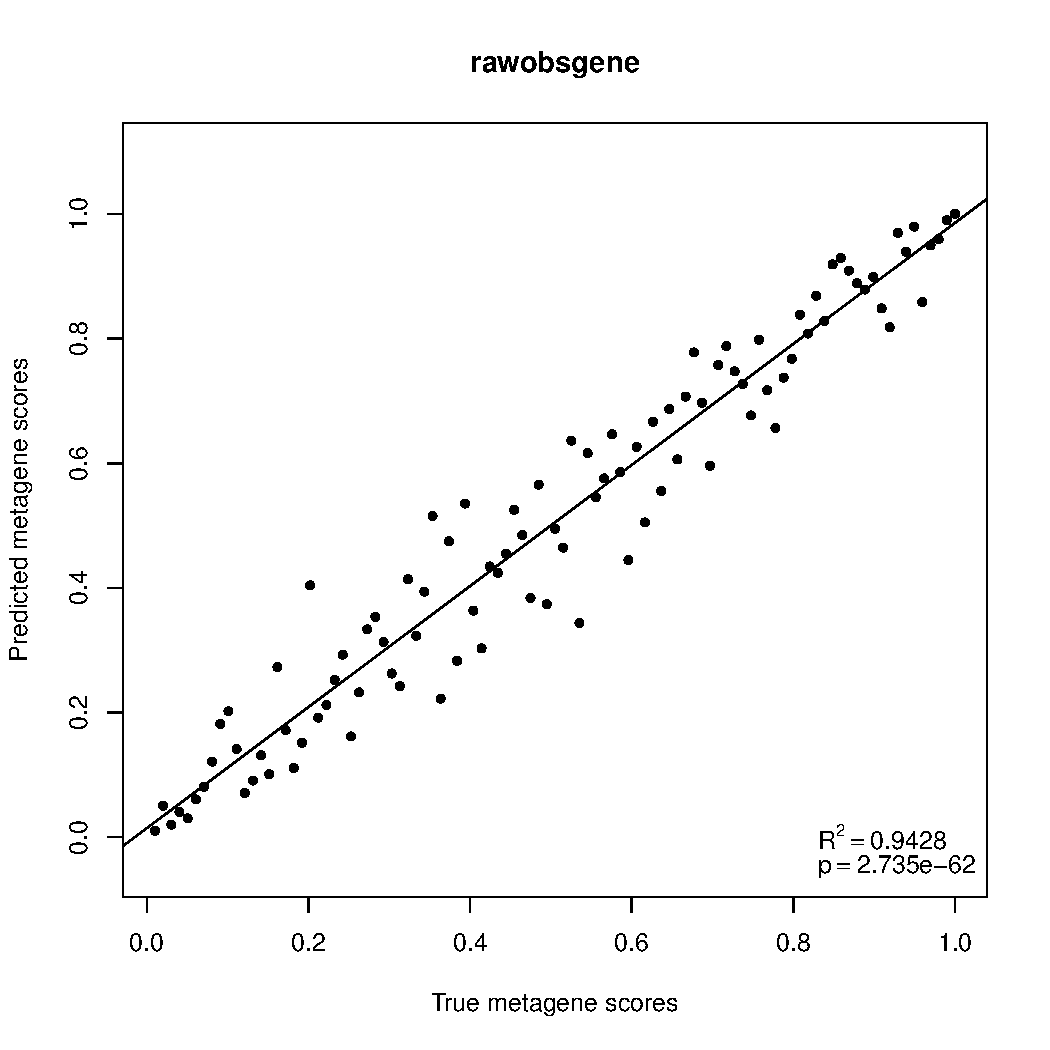
\includegraphics[page=1,width=0.32\linewidth]{results2/stepwise_cris_cris}
	\includegraphics[page=2,width=0.32\linewidth]{results2/stepwise_cris_cris}
	\includegraphics[page=3,width=0.32\linewidth]{results2/stepwise_cris_cris}
	\includegraphics[page=4,width=0.32\linewidth]{results2/stepwise_cris_cris}
	\includegraphics[page=5,width=0.32\linewidth]{results2/stepwise_cris_cris}
	\includegraphics[page=6,width=0.32\linewidth]{results2/stepwise_cris_cris}
	\includegraphics[page=7,width=0.32\linewidth]{results2/stepwise_cris_cris}
	\includegraphics[page=8,width=0.32\linewidth]{results2/stepwise_cris_cris}
	\includegraphics[page=9,width=0.32\linewidth]{results2/stepwise_cris_cris}
	\includegraphics[page=10,width=0.32\linewidth]{results2/stepwise_cris_cris}
	\caption{Comparison of the predicted obesity metagenes with the true obesity metagene in \gls{nzbc} data}
	\label{fig:stepwise_cris}
\end{figure}

\begin{figure}[htpb]
	\centering
	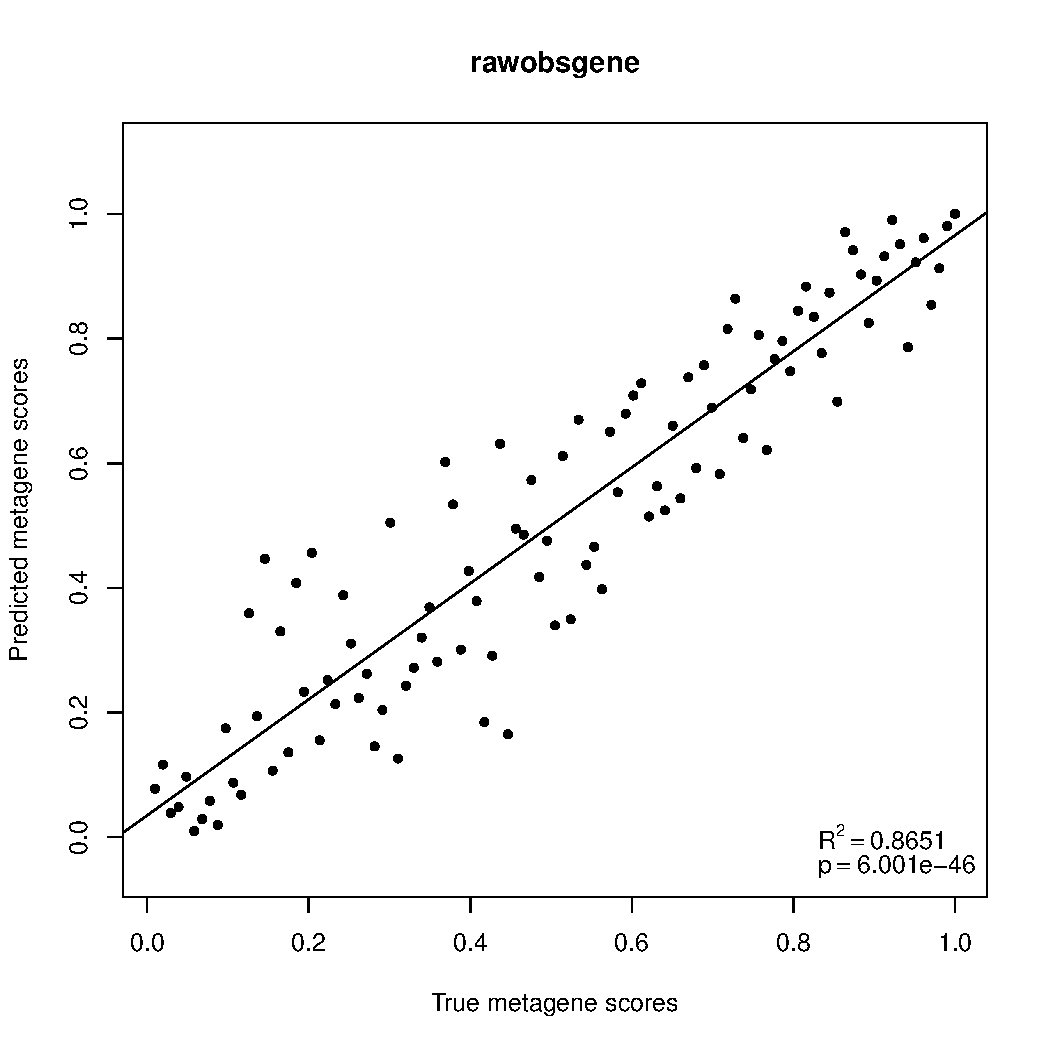
\includegraphics[page=1,width=0.32\linewidth]{results2/stepwise_cr_cris}
	\includegraphics[page=2,width=0.32\linewidth]{results2/stepwise_cr_cris}
	\includegraphics[page=3,width=0.32\linewidth]{results2/stepwise_cr_cris}
	\includegraphics[page=4,width=0.32\linewidth]{results2/stepwise_cr_cris}
	\includegraphics[page=5,width=0.32\linewidth]{results2/stepwise_cr_cris}
	\includegraphics[page=6,width=0.32\linewidth]{results2/stepwise_cr_cris}
	\includegraphics[page=7,width=0.32\linewidth]{results2/stepwise_cr_cris}
	\includegraphics[page=8,width=0.32\linewidth]{results2/stepwise_cr_cris}
	\includegraphics[page=9,width=0.32\linewidth]{results2/stepwise_cr_cris}
	\includegraphics[page=10,width=0.32\linewidth]{results2/stepwise_cr_cris}
	\caption{Comparison of the predicted obesity metagenes with the true obesity metagene in CR data}
	\label{fig:stepwise_cr}
\end{figure}

Taken together, these results suggested that the variables included in these step wise models were associated with the obesity metagenes identified in CR and FM data sets.
However, there were no single common pathway that was present in all of the models; although Akt, \gls{egfr} and \gls{pr} pathway metagenes were frequently included in many of the models.
The role of the pathways included in the models and the possible biological links of these pathways to the obesity metagenes remain unclear, and should be the focus for future investigations.

